%preamble
\documentclass[a4paper,11pt,fleqn,twoside,openright]{memoir} % Brug openright hvis chapters skal starte p� h�jresider; openany, oneside

%%%% PACKAGES %%%%
\usepackage{fourier}   %font
% �� Overs�ttelse og tegns�tning �� %
\usepackage[ansinew]{inputenc}					% G�r det muligt at bruge �, � og � i sine .tex-filer
\usepackage[english]{babel}							% Dansk sporg, f.eks. tabel, figur og kapitel
\usepackage[T1]{fontenc}								% Hj�lper med orddeling ved �, � og �. S�tter fontene til at v�re ps-fonte, i stedet for bmp					
\usepackage{latexsym}										% LaTeX symboler
\usepackage{xcolor,ragged2e,fix-cm}			% Justering af elementer
\usepackage{pdfpages}										% G�r det muligt at inkludere pdf-dokumenter med kommandoen \includepdf[pages=]{fil.pdf}	
\pretolerance=2500 											% G�r det muligt at justre afstanden mellem ord (h�jt tal, mindre orddeling og mere space mellem ord)
\usepackage{ulem}                       % Gennemstregning af ord med koden \sout{}
																			
% �� Figurer og tabeller � floats  �� %
\usepackage{flafter}										% S�rger for at dine floats ikke optr�der i teksten f�r de er sat ind.
\usepackage{multirow}                		% Fletning af r�kker
\usepackage{hhline}                   	% Dobbelte horisontale linier
\usepackage{multicol}         	        % Fletning af kolonner
\usepackage{colortbl} 									% Mulig�re farver i tabeller
\usepackage{here}												% G�r det muligt at placere figurer hvor du vil.   \begin{figure}[!h] % Will not be floating.
\usepackage{wrapfig}										% Inds�ttelse af figurer omsv�bt af tekst. \begin{wrapfigure}{Placering}{St�rrelse}
\usepackage{floatflt}										% Inds�ttelse af tabeller omsv�bt af tekst.
\pdfoptionpdfminorversion=6							% Muligg�r inkludering af pdf dokumenter, af version 1.6 og h�jere
\usepackage{placeins}	
% �� Matematiske formler og maskinkode ��
\usepackage{amsmath,amssymb,stmaryrd} 	% Bedre matematik og ekstra fonte
\usepackage{textcomp}                 	% Adgang til tekstsymboler
\usepackage{mathtools}									% Udvidelse af amsmath-pakken.
\usepackage{eso-pic}										% Tilf�j billedekommandoer p� hver side
\usepackage{lipsum}											% Dummy text \lipsum[..]

% �� PDF og billede optimering �� %
\usepackage{graphicx} 									% Pakke til jpeg/png billeder


\usepackage{lipsum}

\newcommand{\exedout}{%
  \rule{0.8\textwidth}{0.5\textwidth}%
}


% �� Referencer, bibtex og url'er �� %
\usepackage{url}

%% Define a new 'leo' style for the package that will use a smaller font.
\makeatletter
\def\url@leostyle{%
  \@ifundefined{selectfont}{\def\UrlFont{\sf}}{\def\UrlFont{\small\ttfamily}}}
\makeatother
%% Now actually use the newly defined style.
\urlstyle{leo}

\usepackage[english]{varioref}						% Giver flere bedre mulighed for at lave krydshenvisninger
\usepackage{natbib}											% Litteraturliste med forfatter-�r og nummererede referencer


% �� Floats �� %
\let\newfloat\relax 										% Memoir har allerede defineret denne men det g�r float pakken ogs�
\usepackage{float}

\usepackage[marginclue,inline,draft,english,silent]{fixme}			

% Inds�t rettelser og lignende med \fixme{...} Med final i stedet for draft, udl�ses en error for hver fixme, der ikke er slettet, n�r rapporten bygges.

%%%% CUSTOM SETTINGS %%%%

% �� Marginer �� %
\setlrmarginsandblock{3.5cm}{2.5cm}{*}	% \setlrmarginsandblock{Indbinding}{Kant}{Ratio}
\setulmarginsandblock{2.5cm}{3.0cm}{*}	% \setulmarginsandblock{Top}{Bund}{Ratio}
\checkandfixthelayout 									% Laver forskellige beregninger og s�tter de almindelige l�ngder op til brug ikke memoir pakker

%	�� Afsnitsformatering �� %
\setlength{\parindent}{0mm}           	% St�rrelse af indryk
\setlength{\parskip}{3mm}          			% Afstand mellem afsnit ved brug af double Enter
\linespread{1,1}												% Linie afstand

% �� Litteraturlisten �� %
\bibpunct{[}{]}{,}{a}{}{;}					% Definerer de 6 parametre ved Harvard henvisning (bl.a. parantestype og seperatortegn)
\bibliographystyle{bibtex/harvard} 			% Udseende af litteraturlisten

% �� Indholdsfortegnelse �� %
\setsecnumdepth{subsubsection}		 			% Dybden af nummerede overkrifter (part/chapter/section/subsection)
\maxsecnumdepth{subsubsection}					% �ndring af dokumentklassens gr�nse for nummereringsdybde
\settocdepth{subsection} 								% Dybden af indholdsfortegnelsen

% �� Visuelle referencer �� %
\usepackage[colorlinks]{hyperref}			 	% Giver mulighed for at ens referencer bliver til klikbare hyperlinks. .. [colorlinks]{..}
\hypersetup{pdfborder = 0}							% Fjerner ramme omkring links i fx indholsfotegnelsen og ved kildehenvisninger ��
\hypersetup{														%	Ops�tning af hyperlinks
    colorlinks = false,
    linkcolor = black,
    anchorcolor = black,
    citecolor = black
}

\definecolor{gray}{gray}{0.80}					% Definerer farven gr�

% �� Ops�tning af figur- og tabeltekst �� %
 	\captionnamefont{
 		\small\bfseries\itshape}						% Ops�tning af tekstdelen ("Figur" eller "Tabel")
  \captiontitlefont{\small}							% Ops�tning af nummerering
  \captiondelim{. }											% Seperator mellem nummerering og figurtekst
  \hangcaption													%	Venstrejusterer flere-liniers figurtekst under hinanden
  \captionwidth{\linewidth}							% Bredden af figurteksten
	\setlength{\belowcaptionskip}{10pt}		% Afstand under figurteksten

% �� Sidehoved �� %
\pagestyle{plain}
		
% �� Navngivning �� %
\addto\captionsenglish{
%	\renewcommand\appendixname{Bilag}
	\renewcommand\contentsname{Table Of Contents}	
%	\renewcommand\appendixpagename{Bilag}
	\renewcommand\cftchaptername{\chaptername~}
%	\renewcommand\cftappendixname{\appendixname~}
%	\renewcommand\appendixtocname{Bilag}
}
%Appendix ops�tning. Toc er s�tter appendix kapitlerne i indholdfortegnelsen og head s�tter en overskrift til appendix kapitlet

\usepackage{appendix}
%\usepackage[toc,page]{appendix}


% �� Kapiteludssende �� %

\definecolor{numbercolor}{gray}{0.7}
\newif\ifchapternonum

\makechapterstyle{jenor}{
  \renewcommand\printchaptername{}
  \renewcommand\printchapternum{}
  \renewcommand\printchapternonum{\chapternonumtrue}
  \renewcommand\chaptitlefont{\fontfamily{pbk}\fontseries{db}\fontshape{n}\fontsize{25}{35}\selectfont\raggedleft}
  \renewcommand\chapnumfont{\fontfamily{pbk}\fontseries{m}\fontshape{n}\fontsize{1in}{0in}\selectfont\color{numbercolor}}
  \renewcommand\printchaptertitle[1]{%
    \noindent
    \ifchapternonum
    \begin{tabularx}{\textwidth}{X}
    {\let\\\newline\chaptitlefont ##1\par}
    \end{tabularx}
    \par\vskip-2.5mm\hrule
    \else
    \begin{tabularx}{\textwidth}{Xl}
    {\parbox[b]{\linewidth}{\chaptitlefont ##1}} & \raisebox{-15pt}{\chapnumfont \thechapter}
    \end{tabularx}
    \par\vskip2mm\hrule
    \fi
  }
}

\chapterstyle{madsen}

% �� Fjerner den vertikale afstand mellem listeopstillinger og punktopstillinger �� %
\let\olditemize=\itemize							
\def\itemize{\olditemize\setlength{\itemsep}{-1ex}}
\let\oldenumerate=\enumerate						
\def\enumerate{\oldenumerate\setlength{\itemsep}{-1ex}}


%%%% CUSTOM COMMANDS %%%%

% �� Billede hack �� %
\newcommand{\figur}[4]{
		\begin{figure}[H] \centering
			\includegraphics[width=#1\textwidth]{billeder/#2}
			\caption{#3}\label{#4}
		\end{figure}
}

% �� Specielle tegn �� %
\newcommand{\celcius}{^{\circ}C}
\newcommand{\gr}{^{\circ}}
\newcommand{\g}{\cdot}

% �� Promille-hack (\promille) �� %
\newcommand{\promille}{%
  \relax\ifmmode\promillezeichen
        \else\leavevmode\(\mathsurround=0pt\promillezeichen\)\fi}
\newcommand{\promillezeichen}{%
  \kern-.05em%
  \raise.5ex\hbox{\the\scriptfont0 0}%
  \kern-.15em/\kern-.15em%
  \lower.25ex\hbox{\the\scriptfont0 00}}


%%%% ORDDELING %%%%

\hyphenation{hvad hvem hvor MPa kon-se-kvens-klas-se bj�l-ken byg-ning-er e-le-ment brud-li-ni-er frem-l�bs-tem-pe-ra-tur-en Bj�l-ker-ne ind-be-ret-tel-se be-hand-ler-en ana-ly-se stig-ning-en h�nd-el-ser in-te-res-sen-ter-ne f�lg-en-de in-te-res-sen-ter in-te-res-sent-ana-ly-sen pro-blem-for-mu-le-ring pro-ble-mer pro-ble-ma-tisk kraft-y-del-ser vur-de-rer grebs-styr-ke da-ta-ana-ly-se sundheds-sektor u-sande grebs-styrke} 
\usepackage{booktabs} %skal bruges hvis der bruges PDF2LaTEX             
\definecolor{headerColor}{RGB}{44, 39, 101}
%preamble slut
\begin{document}

\includepdf{Frontpage.pdf}
\cleardoublepage
%\clearpage
%\cleardoublepage 
% Dette er LaTeX-versionen af titelbladet for TNB studenterrapporter
% Filen kr�ver:
% Universitetets logo:  AAU-logo-stud-UK eller AAU-logo-stud-DK
% Synopsis: En fil ved navn synopsis.tex

% Udarbejdet af: Jesper N�rgaard (jesper@noergaard.eu) 10. april 2012

\phantomsection
\pdfbookmark[0]{Titelblad}{titelblad}
\thispagestyle{empty}

\begin{minipage}{0.55\textwidth}
	
\includegraphics{Images/AAU_LOGO_RGB_OWN.png}
\end{minipage}
\begin{minipage}{0.35\textwidth}
\vspace*{0.25cm}
{\textbf{\textcolor{headerColor}{Department of Architecture,}}}\\
{ \textbf{ \textcolor{headerColor}{Design and Media Technology}}}\\
%{\small  Rendsburggade 14} \\
%{\small 9000 Aalborg} \\
%{\small Phone: +45 99 40 87 93} \\
%{\sf\small Fax 98 13 63 93} \\\\
\newline
{  \textcolor{headerColor}{Medialogy, 10th Semester}}
\end{minipage}

\vspace*{1cm}

\begin{minipage}[t]{0.48\textwidth}
\textbf{Title:}  %\\[2pt]\bigskip\hspace{2ex} 
\newline
Supporting Self-tracking in Telehealth \newline

\textbf{Project Period:} %\\[5pt]\bigskip\hspace{2ex}
\newline
Spring 2016 \newline

\textbf{Semester Theme:} %\\[5pt]\bigskip\hspace{2ex}
\newline
 \newline

\textbf{Supervisor:} %\\[5pt]\hspace*{2ex}
\newline
Hendrik Knoche\newline
%\vspace*{1cm}

\textbf{Project group no.}\newline
161039\newline


\textbf{Members:} \\

\underline{\hspace*{5cm}} \\
Stephanie Githa Nadarajah \\

\underline{\hspace*{5cm}} \\
Peder Walz Pedersen \\



\textbf{Number of copies:} 3 \\
\textbf{Page numbers:} ?? \\
\textbf{Finished on:} May $25^{th}$ 2016

\end{minipage}
\hfill
\begin{minipage}[t]{0.483\textwidth}
\textbf{Abstract:} \\[5pt]
\mbox{\parbox{7cm}{\bigskipA stoma nurse has an important role in educating a patient to adjust to the new lifestyle after a stome surgery by teaching the patient self-management skills, also called stoma self-care. Stoma self-care is acknowledged as a crucial factor in determining a patient's quality of life after a surgery. The Urostomy Education Scale (UES) is a standardized educational intervention that aims to facilitate the nurses in teaching patients stoma self-care. It is intended to improve quality of stoma care and reduce random clinical practice. Despite of the many advantages of the UES, the current implementation in practice does not support nurses in teaching stoma self-care to patients using the UES. Challenges include missing overview of patient's progression, portability and availability of the patient's data. In this project, we designed and implemented an application to tablet devices that based on the UES facilitates the nurse in teaching the patients self-management skills. Through an iterative design and prototyping process, we found that mobile technology opens up for new perspectives to improve quality of care for stoma patients.  \bigskip}}
\end{minipage}

\vfill

{\footnotesize\itshape Copyright@2016. This report and/or appended material may not be partly or completely published or copied without prior written approval from the authors. Neither may the contents be used for commercial purposes without this written approval.}

% Rapportens indhold er frit tilg�ngeligt, men offentligg�relse (med kildeangivelse) m� kun ske efter aftale med forfatterne.
% The content of the report is freely available, but publication (with source reference) may only take place in agreement with the authors.
 %synopsis
\cleardoublepage
%---------Preface---------------
\chapter{Preface}

The following internship report was developed during Autumn 2015 on the ninth semester of Medialogy at Aalborg University. The main theme for the project was \textit{Media Innovation} with main focus on understanding and analysing elements in human centred interaction, using relevant methods to design solutions and implementing an interactive system based on a design solution. 

\section*{Reading Guide}
In the report, all the source references are gathered in the \textit{Bibliography} chapter, listed using the Harvard system of referencing. In the body text, a source is cited as [Surname, Year of publication]. The full details of the given source can be found in the reference chapter with the following information: \textit{Author, title and publisher}. Web pages are referenced with: \textit{Author, title and data}.

Figures and tables are numbered in accordance with chapter number. For instance, the first figure in Chapter 4 has the number 4.1., the second figure has the number 4.2., etc. Each figure and table is referred to in the body text and given an explanatory text in addition to the numbering. Abbreviations are introduced in their extended form the first time they appear. Enclosed with this report is a CD containing the full report, process analysis, appendices, internship diary and other extra materials. 

\section*{Thanks}
Thanks are given to stoma nurse researchers Bente T. Jensen, Susanne A. Kristensen for making it possible for us to work on this project. Also a special thanks to project managers Klaus V. Kristensen and Lina Gotfredsen for giving me the opportunity to be a part of APPlab and providing supervision and assistance in this project and many other projects in APPlab. Special thanks are given to current and previous interns and students at APPlab for their collaboration, assistance and feedback. 
\cleardoublepage

\begin{KeepFromToc}
	\tableofcontents
\end{KeepFromToc}

\chapter{Motivation}
In recent years, the proportion of chronically ill patients has increased in accordance with an expanding elderly population \citep{motWHO}. By 2030 the World Health Organization (WHO) has predicted that Chronic Obstructive Pulmonary Disease (COPD) will affect over 64 million people and will be the third leading cause of death worldwide \citep{motStat}. 

COPD is a progressive lung disease in which the airways are damaged, resulting in periods of exacerbations among those affected. An exacerbation can be defined as \textit{"a sustained worsening of the patient's condition, from the stable state and beyond normal day-to-day variations, that is acute in onset and necessitates a change in regular medication in a patient with underlying COPD"} \citep{motExace}, where the worsening of the patient's condition refers to a worsening in symptoms or lung function. Patients with COPD experience symptoms, such as shortness of breath (known as dyspnea), phlegm, cough, wheezing and chest tightness \citep{motSymp}. 
 
 Research shows that delayed treatment following the onset of an exacerbation results in increased use of healthcare services, readmission to the hospital and a decline in health-related quality of life \citep{motExace}. Early detection and treatment of exacerbations are therefore an important step towards preventing decline in patients' quality of life and healthcare utilisation.  



%[1] Global Health and Aging, World Health Organization & National Institute on Aging and National Institutes of Health, 2011.
%
%[2] World Health Organization. Department of Measurement and Health Information Systems of the Information, Evidence and Research Cluster. 2008. World Health Statistics 2008. World Health Organization.
%
%[3] Kessler, R., Partridge, M. R., Miravitlles, M., Cazzola, M., Vogelmeier, C., Leynaud, D., & Ostinelli, J. (2011). Symptom variability in patients with severe COPD: a pan-European cross-sectional study. European Respiratory Journal, 37(2), 264-272.
%
%[4] Rodriguez-Roisin, R. (2000). Toward a consensus definition for copd exacerbations*. CHEST Journal, 117(5_suppl_2), 398S-401S.
%
%[5] Wilkinson, T. M., Donaldson, G. C., Hurst, J. R., Seemungal, T. A., & Wedzicha, J. A. (2004). Early therapy improves outcomes of exacerbations of chronic obstructive pulmonary disease. American journal of respiratory and critical care medicine, 169(12), 1298-1303.
%
%[6] Field, M. J. (Ed.). (1996). Telemedicine: A guide to assessing telecommunications for health care. National Academies Press.
%
%[7] Pedone, C., & Lelli, D. (2015). Systematic review of telemonitoring in COPD: an update. Pneumologia i Alergologia Polska, 83(6), 476-484.
%
%[8] Pennebaker, J. W. (2000). Psychological factors influencing the reporting of physical symptoms. The science of self-report: Implications for research and practice, 299-315.
%
%[9] Ure, J., Pinnock, H., Hanley, J., Kidd, G., Smith, E. M., Tarling, A., ... & McKinstry, B. (2011). Piloting tele-monitoring in COPD: a mixed methods exploration of issues in design and implementation. Primary Care Respiratory Journal, 21(1), 57-64.
%
%[10] Bestall, J. C., Paul, E. A., Garrod, R., Garnham, R., Jones, P. W., & Wedzicha, J. A. (1999). Usefulness of the Medical Research Council (MRC) dyspnoea scale as a measure of disability in patients with chronic obstructive pulmonary disease. Thorax, 54(7), 581-586.
%
%[11] Kendrick, K. R., Baxi, S. C., & Smith, R. M. (2000). Usefulness of the modified 0-10 Borg scale in assessing the degree of dyspnea in patients with COPD and asthma. Journal of Emergency Nursing, 26(3), 216-222.
%
%[12] Gift, A. G. (1989). Validation of a vertical visual analogue scale as a measure of clinical dyspnea. Rehabilitation Nursing, 14(6), 323-325.
%
%[13] Corbishley, P., & Rodríguez-Villegas, E. (2008). Breathing detection: towards a miniaturized, wearable, battery-operated monitoring system. Biomedical Engineering, IEEE Transactions on, 55(1), 196-204.
%
%[14] Hung, P. D., Bonnet, S., Guillemaud, R., Castelli, E., & Yen, P. T. N. (2008, May). Estimation of respiratory waveform using an accelerometer. In Biomedical Imaging: From Nano to Macro, 2008. ISBI 2008. 5th IEEE International Symposium on (pp. 1493-1496). IEEE.
%
%[15] Kawamoto, K., Tanaka, T., & Kuriyama, H. (2014, September). Your activity tracker knows when you quit smoking. In Proceedings of the 2014 ACM International Symposium on Wearable Computers (pp. 107-110). ACM.
%
%[16] Schlecht, N. F., Schwartzman, K., & Bourbeau, J. (2005). Dyspnea as clinical indicator in patients with chronic obstructive pulmonary disease. Chronic respiratory disease, 2(4), 183-191.
%
%[17] Okubo, M., Imai, Y., Ishikawa, T., Hayasaka, T., Ueno, S., & Yamaguchi, T. (2009). Development of automatic respiration monitoring for home-care patients of respiratory diseases with therapeutic aids. In 4th European Conference of the International Federation for Medical and Biological Engineering (pp. 1117-1120). Springer Berlin Heidelberg.
%
%[18] Colantonio, S., Dellacà, R. L., Govoni, L., Martinelli, M., Salvetti, O., & Vitacca, M. (2012). A Decision Making Approach for the Remote, Personalized Evaluation of COPD Patients’ Health Status. Proc. 7th Int. W. BSI, 2-4.
%
%[19] Chan, M., Estève, D., Fourniols, J. Y., Escriba, C., & Campo, E. (2012). Smart wearable systems: Current status and future challenges. Artificial intelligence in medicine, 56(3), 137-156.
%
%[20] Davis, F. D. (1989). Perceived usefulness, perceived ease of use, and user acceptance of information technology. MIS quarterly, 319-340.


\chapter{The COPD-patient}


\chapter{Telehealth for COPD}
%
% FROM PROPOSAL:
%

Telehealth (support of health care using electronic information and communication technologies when patient and provider are in a separate location) can play an important role in early detection and treatment of exacerbations. 

In spite of the interest telehealth interventions have gained, studies have produced conflicting results regarding the effectiveness of telehealth interventions \citep{pedone}. One of the factors that may be linked to the cause of telehealth interventions failing to detect exacerbations early, can be addressed to difficulties assessing symptoms through self-report. Previous studies support this finding and further report that binary self-report measures are not always intuitive for patients, who are constantly symptomatic \citep{pedone}. Since physical symptoms are influenced by psychological and individual processes \citep{pennebakker}, self-reported binary measures might be biased and further not capture the relevant features necessary for clinical decision making.  


%
% FROM LONG DRAFT:
%

%
%Chronic Obstructive Pulmonary Disease (COPD) is a progressive lung disease in which the airways are damaged and patients have to cope with various different symptoms, such as shortness of breath (known as dyspnea), phlegm, cough, wheezing and/or chest tightness \cite{Kessler}. Exacerbations  - a worsening in patients’ lung function or symptoms - are a major problem with COPD. Delayed treatment following their onset increased use of healthcare services, readmission to the hospital and a decline in health-related quality of life \cite{Wilkinson}. Early detection and treatment of exacerbations are therefore an important step towards preventing decline in patients’ quality of life and healthcare utilisation.
%
%Telehealth systems that allows for remote monitoring of patients using information and communication technologies are widely used today for the purpose of early detection and treatment of exacerbations in COPD. In telehealth, patients collect both objective (e.g. oxygen saturation) and subjective data (e.g. binary answers to whether there is an increase in dyspnea more than usual). The collected data is transmitted to healthcare providers (usually trained nurses) who review it. Based on an individual “normal range” defined by a healthcare provider, the system flags data for follow-ups in which healthcare providers contact the patient, if needed to advise on potential initiation of treatment. Despite the gained interest in telehealth interventions, studies have produced conflicting results regarding their effectiveness \cite{Pedone}. 


%In the context of chronically ill healthcare providers implement telehealth systems to communicate remotely with patients, when they are out of clinic. Telehealth systems require active participation of patients to collect objective and subjectively assessed data that are directly related to a health condition. While the health domain literature typically focuses only on the comparison of effectiveness of telehealth systems with standard care approaches, literature shows several user needs and concerns that needs to be addressed, when developing self-tracking tools. These user needs have not been investigated in the telehealth domain. We conducted a study on COPD patients who used a state of the art telehealth solution to addresses this gap. 

%While telehealth can be categorized as a form of prescribed self-tracking, it is a special case, given that patients are monitored by a healthcare provider and mandated to self-track. 

\begin{figure}[!h] \centering
			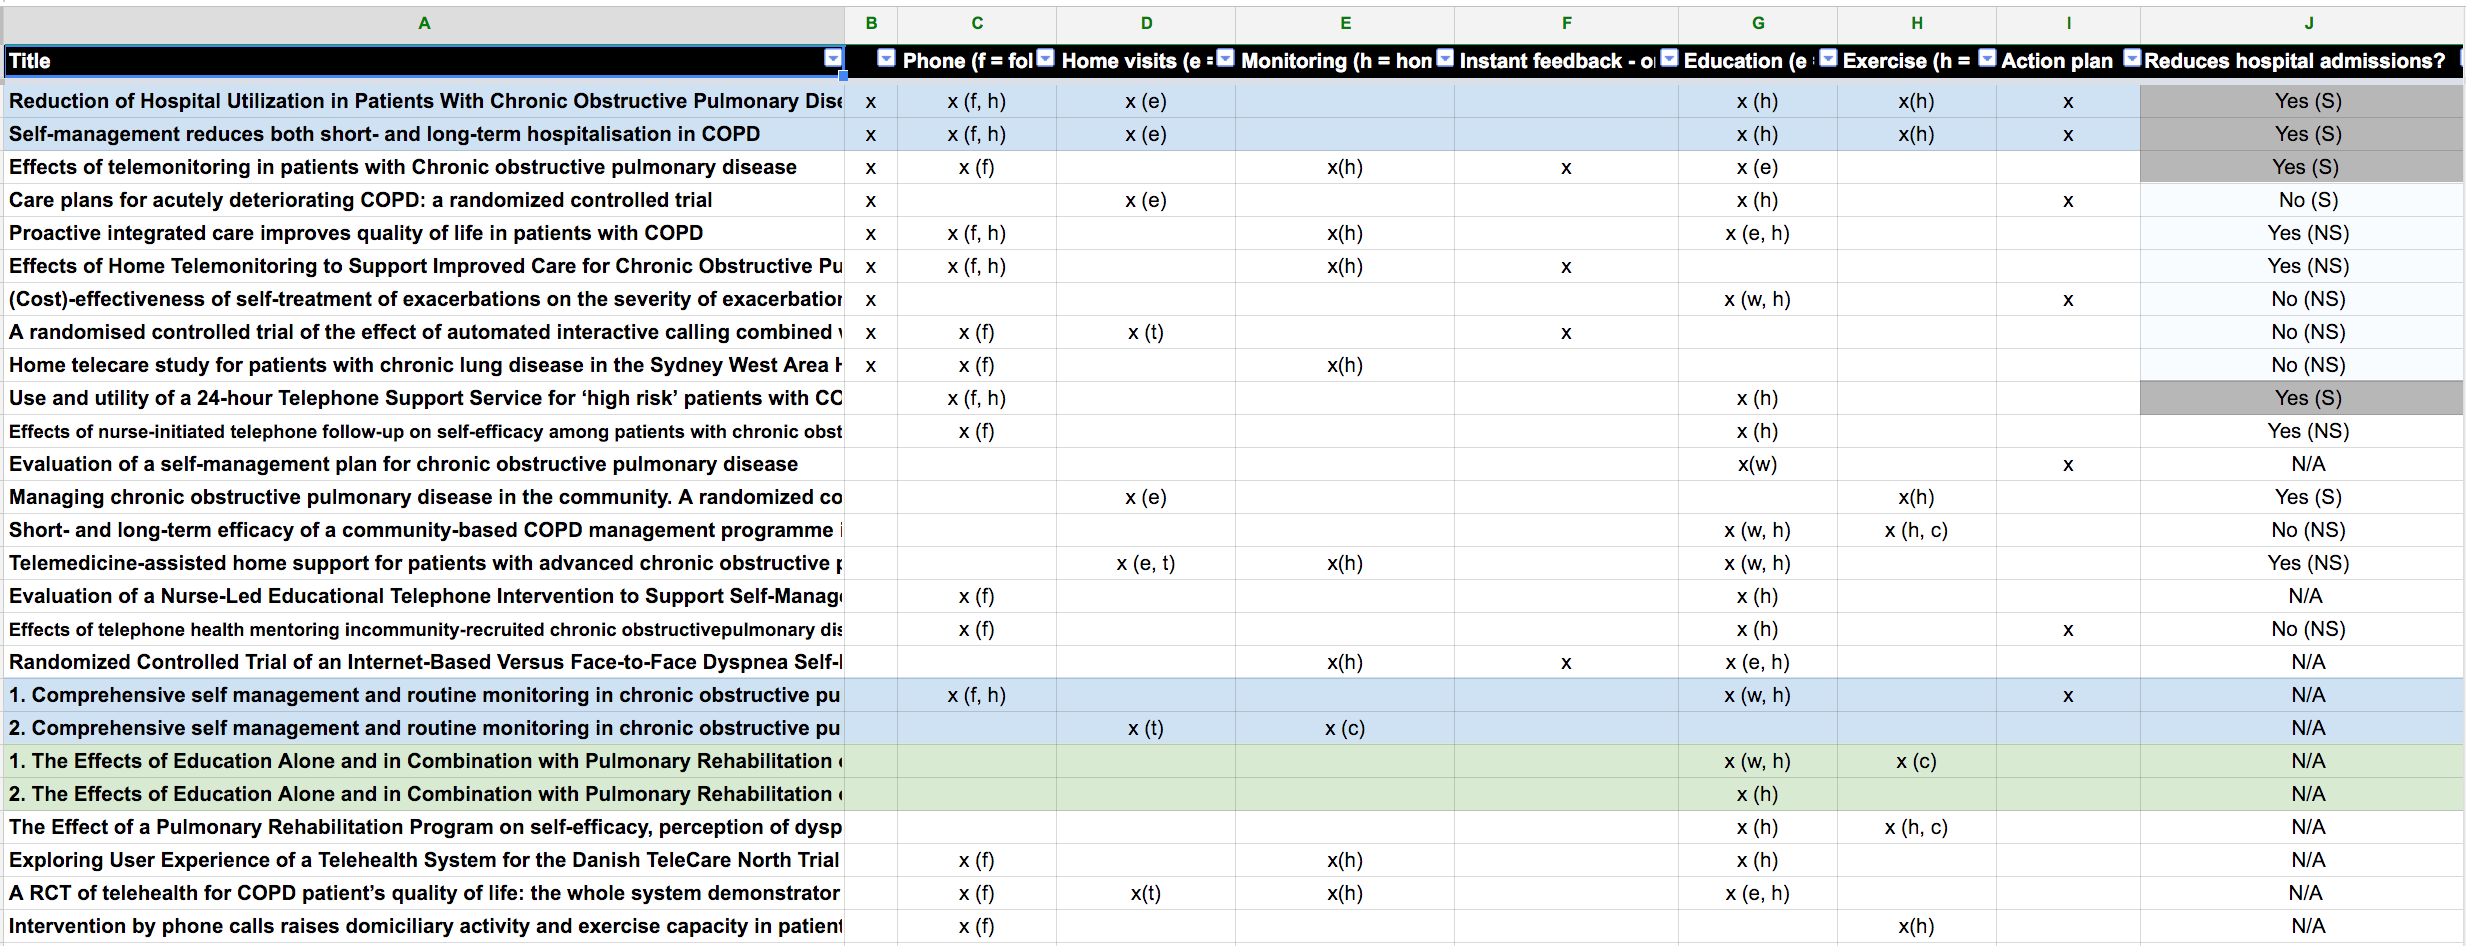
\includegraphics[width=1\textwidth]{Images/telehealth/thInitial.png}
		\caption{Research table with health-related outcomes of telehealth interventions} \label{fig:thInitial}
\end{figure}

\section{Current Literature}
We made an extensive review on telehealth literature and found little on how telehealth systems have been designed to patients needs (See research tables on CD). Current literature primarily shows health-related outcomes of telehealth interventions in comparison with standard care. We compared outcomes from different studies on telehealth studies (See Figure \ref{fig:thInitial}) and found conflicting results due to a wide range of different interventions used. From this it is difficult to assess what has an effect.

\section{State of the Art}
 hjkh
\section{Interviews with Healthcare Professionals}


\chapter{Personal Informatics}
In Personal Informatics people collect different kinds of personal data voluntarily for the purpose of self-reflection and gaining knowledge about themselves \cite{Li2010}.  Personal Informatics have identified various aspects of self-tracking activities \cite{Li2010} and since self-tracking is a common denominator to the fields of both telehealth and Personal Informatics we (in the absence of technology knowledge in telehealth) use the literature of Personal Informatics as an analytical lens for the field of telehealth. We analyse the literature of Personal Informatics for different drivers for self-tracking, how people track and the barriers that typical arise in self-tracking activities. We distinguish between self-tracking that is initiated by oneself (henceforth referred to as discretionary tracking) and self-tracking initiated by a healthcare provider (henceforth referred to as prescribed tracking). While discretionary trackers take up self-tracking voluntarily, prescribed trackers are either recommended or required to track by a healthcare provider (i.e. a physician or a nurse), e.g. for a specific treatment, for long-term performance or approval for surgery. Common to both discretionary and prescribed self-trackers is that they collect data related to their health and well-being \citep{Choe2014, MacLeod2014, Chung2016}.



\section{Why People Track} 
From the literature, we classified main motivations for self-tracking into five categories.

\paragraph{Documentation:}
Some discretionary trackers are mainly interested in documenting their activities, rather than changing them \citep{Rooksby2014}. Self-tracking not for one's own purpose, but partly or largely to create records for the healthcare providers was a reason for imposed self-tracking in \citep{Ancker2015}. 

\paragraph{Life Experience} 
People tracking for life experience are mainly discretionary trackers who track out of natural curiosity about what their data might reveal about themselves \citep{Li2010, Epstein2015} or because of an interest in quantitative data \citep{Li2010, Rooksby2014}. Others aim to discover new tools or because of an interest in gadgets and technology \citep{Li2010, Rooksby2014}. 

\paragraph{Communication} 
Discretionary trackers tracking for documentation also used the data as a way of underscoring their effort through sharing, e.g. using a pedometer to convince a friend that they walked a lot \citep{Rooksby2014}. Others used it for direct social benefits (for practical reasons e.g. informing others about their location, for social engagement, etc. \citep{Epstein2015}) and in response to gamification incentives, such as to score points or achievements \citep{Rooksby2014}. Some self-trackers with a health-related condition use tracking to seek recognition from their healthcare provider. They also use it as evidence when they find empathy of healthcare providers lacking, or in order to show a complete picture of their life, when they do not find measurements taken in the clinic sufficient \citep{Chung2016}. Some hope that self-tracking can help communicate their condition to family members \citep{MacLeod2014}. 

\paragraph{Self-Knowledge} \label{selfknowledge}
Self-trackers in this category track to get a sense of the current state of their condition \citep{MacLeod2014, Ancker2015}. Some are motivated to track in order to identify potential links between different factors, e.g. tracking medication and diet to identify what caused stomach problems \citep{Rooksby2014}. They also self-track in order to learn what to add in their lives, in order to prevent undesirable health-related episodes (e.g. initiating medication to prevent a worsening of condition) or what to remove in order to reduce impact of such episodes (e.g. stop smoking to reduce symptom severity) \citep{MacLeod2014}. These motives indicate that this type of self-trackers are also partially motivated to self-improve. 

\paragraph{Self-Improvement} \label{selfimprove}
Common to these self-trackers is a desire to change or maintain a behaviour in order to improve their well-being or lifestyle \citep{MacLeod2014, Ancker2015, Chung2016, Li2011, Whooley2014}. Self-trackers in this category are goal-driven (e.g. have the goals "avoid drinking coffee X hours before sleeping" or "run three times a week") and regulate their progress towards their goal \citep{Chung2016, Rooksby2014, Li2011}. MacLeod et al. found that prescribed self-trackers were motivated due to the resulting self-efficacy and sense of agency. Tracking made them feel they were helping managing their condition and empowered to take control of their own health. Despite being initiated to self-track by their provider, a majority of the self-trackers were motivated to continue self-tracking even after their provider did not require it anymore \citep{MacLeod2014}. 

\section{How People Track}
Researchers have proposed different models for understanding, how self-trackers concretely use personal informatics systems over time. Li et al. proposed a five-staged model describing, how self-trackers transition between these stages: (1) \textit{preparation} (user determines what and how to track data), (2) \textit{collection} (user tracks data), (3) \textit{integration} (user prepares data for reflection), (4) \textit{reflection} (user explores data to gain self-knowledge) and (5) \textit{action} (user decides what to do with newfound self-knowledge) \citep{Li2010}. The \textit{reflection} stage can further be divided into \textit{maintenance} and \textit{discovery} \citep{Li2011}. Opposed to the \textit{maintenance} phase, self-trackers in the \textit{discovery} phase do either not know their goal and/or have not identified important factors yet to determine appropriate actions \citep{Li2011}. 

Epstein et al. divided the \textit{preparation} stage into \textit{deciding} and \textit{selecting}. Self-trackers first decide to track and then select a tool to support their self-tracking efforts \citep{Epstein2015}. Li et al. describe the five-staged model as linear \citep{Li2010}, whereas Epstein et al. further describe \textit{tracking} and \textit{acting} as ongoing processes of collecting, integrating and reflecting. Epstein et al. do not separate collecting, integrating and reflecting into stages as these activities can and do occur simultaneously \citep{Epstein2015, MacLeod2014}. Epstein et al.'s model was developed using almost the same methods as Li et al. though (according to the authors) conducted on a more general population (recruited from an online crowdsourcing marketplace) \citep{Epstein2015}. The \textit{integration} stage can be more or less apparent to the self-tracker depending on type of personal informatics system. Both Whooley et al. and Li et al. write about two types; system-driven and user-driven. In a user-driven personal informatics system the self-tracker is responsible for the activities involved (e.g. aggregating and analysing data) in contrast to system-driven personal informatics system where the system is responsible of the activities, thus requiring less effort of the self-tracker \citep{Whooley2014,Li2010}. Epstein et al. further included stages of \textit{lapsing} and \textit{resuming} into their model, accounting for users sometimes stopping to track for either longer or shorter periods (for instance because of forgetting to track and skipping maybe already known data) and the opportunity of resuming tracking later \citep{Epstein2015}. The nature of lapsing and resuming during self-tracking was also confirmed by \citep{Rooksby2014}. 

We use Epstein et al.'s model as a lens to discuss our own findings on user needs and concerns in the following section. 

\subsection{Deciding and Selecting}
\paragraph{Preparation}
In the \textit{preparation} stage, people decide what to track and how they want to track. One common problem people experience is not always knowing what to track or what questions to ask \citep{Li2011, Choe2014, Chung2015, Patel2012}. Discretionary trackers might not have identified what goals they are trying to meet and/or might not have identified what factors influence their behaviour (\textit{discovery} phase). This means that after an initial phase of tracking, they might have to redefine what to track and what questions to ask \citep{Choe2014}. This mirrors  Li et al.'s findings on self-trackers tending to transition between the \textit{maintenance} and \textit{discovery} phase \citep{Li2011}. 

Prescribed trackers experience that healthcare providers recommend symptom tracking, but sometimes give little support on what to track and how to track (e.g. frequency of tracking) \citep{Patel2012}. Some health conditions involve many symptoms that sometimes arise unexpectedly. Patel et al. found that patients who experienced symptoms that providers had not suggested tracking, had to figure out themselves, whether these symptoms were important and if additional tracking was needed \citep{Patel2012}. Tracking the wrong data or not tracking well enough to gain benefits can according to healthcare providers lead to loss of motivation to keep tracking \citep{Chung2015}.  

Both Patel et al. and Chung et al. found that tools recommended for self-tracking by healthcare providers did not always meet the needs of the self-trackers e.g. tracking symptoms self-trackers want to track \citep{Patel2012, Chung2016}. As a result, self-trackers found other tools or designed their own tracking systems, such as notebooks, health diaries and specific applications. If these tools did not support collaborative review or other requirements from the healthcare provider, it sometimes created tension between patients and providers later in the \textit{reflection} stage \citep{Chung2016}. 

\subsection{Tracking and Acting}					
\paragraph{Collection:}
In the \textit{collection} stage self-trackers collect data about themselves. 

Even though self-trackers do not know how to track well or accurately enough \citep{Chung2015, Patel2012}, they develop their own systems for tracking. Prescribed trackers are only offered little support from health care providers, but do not know how to improve their systems. The self-developed systems are often cumbersome and incomplete and prescribed trackers who choose to track a breadth of health issues pose a significantly challenge on themselves \citep{Patel2012}. Self-tracking too many things can lead to tracking fatigue \citep{Choe2014}. 

Rooksby et al. questioned that people could or always wanted to do rational data collection \citep{Rooksby2014}, which leads to measures with low reliability. Self-trackers skipped tracking when data entries were too long or when data was known beforehand they did not always see the benefit of tracking it \citep{Epstein2015}. Self-trackers might also simply forget to track \citep{Li2010}. 

Prescribed self-trackers found tracking time consuming and requiring effort \citep{Ancker2015} hampering incorporation of tracking into daily routines \citep{Verdezoto2015, Ancker2015}. Self-trackers do not want to spend too much time on entering data \citep{Choe2013, Li2010}. This not only due to act of entering data but includes preparation to do so. For example, resting a number of minutes before taking blood pressure measures increased time and effort \citep{Verdezoto2015}. Incorporation difficulties lead to skipped primary tracking and secondary data, e.g, whether guidelines had been followed by  smoking before taking a blood pressure reading. This reduced reliability and difficulties in data interpretation \citep{Verdezoto2015}. Among prescribed self-trackers, measurements were found not to be clinically useful because of insufficient frequency and detail in tracking \citep{Chung2015}. 

Some subjective measurements also affect the reliability of the data. For instance, when a self-tracker subjectively quantifies expended calories when lifting weights or when self-trackers are required to subjectively assess without any standard (e.g. when wanting to rate relationship satisfaction and ratings are not consistent) \citep{Li2010}. \citep{piloting} suggests similar problems, where prescribed self-trackers subjectively assessed, whether they coughed more or experienced more dyspnea than usual. Some found it difficult to assess such questions, as they were constantly symptomatic and were in doubt of what standard they should compare them to. Data granularity impeded collection when self-trackers were overthinking, while trying to rate mood on a scale from 0 to 10 \citep{Oh2015}. 

Recall bias can reduce data reliability as prescribed trackers did not use a tool for tracking but relied on memory \citep{Patel2012} or postponed manually entering data \citep{MacLeod2014}. Self-trackers who do not enter data immediately or at specific times each day are less likely to remember making the tracking and they are also less confident in the accuracy of their own data \citep{MacLeod2014}. \citep{Li2010} found that one participant problematized the fact that s/he did not have ready access to her tracking device (a computer) at the time symptoms happened. Some prescribed self-trackers appreciate doing tracking in a notebook because of its portability even though it provides little structure \citep{MacLeod2014}. Patel et al. tried to improve the reliability of the data and decrease recall bias by developing a smartphone application enabling prescribed self-trackers to do manual realtime tracking with use of self check-ins for logging symptoms. According to their qualitative evaluation their app was successful but new user needs emerged \citep{Patel2012}. Prescribed self-trackers appreciate the ability to collect a variety of data \citep{MacLeod2014, Patel2012}, which is why prescribed self-trackers appreciate flexibility of notebooks \citep{MacLeod2014} and fortunately the smartphone application by Patel et al. supported prescribed self-trackers in tracking self-selected variables on a 0 to 4 scale, but some participants made a workaround to generate new units that were not initially supported, e.g. "took all pills". The authors report that their smartphone application was engaging, but it still required a great deal of effort for users to track. They end up recommending further simplification within tracking for instance by voice commands \citep{Patel2012}. Another study tried to simplify tracking with use of an Android interactive widget, which allowed easy input of data. The widget was accompanied by an associated app in one condition and another condition, where they only had the app for inputting data. Participants in the condition utilized with the widget had a significantly higher adherence and they also captured an event significantly closer to its actual time than participants in the non-widget condition \citep{Choe2015}. 

\paragraph{Integration:}
In this stage the personal data is "prepared combined and transformed for the user to reflect on" \citep{Li2010}, which involves data aggregation, data analysis, statistical tests and creation of data representations \citep{Li2010}. 

Self-trackers that collect data with pen and paper face a problem, because they have to transcribe data into an electronic format, in order to visualize their data. Self-trackers has to do many things in order to prepare the data for reflection \citep{Li2010}, but if the integration is system-driven less effort is required by the self-tracker \citep{Li2011, Whooley2014} making integration less apparent. There are different trade-offs in the integration stage, depending on whether the system is system-driven or user-driven. User-driven systems expect the user to be able to analyse the data and ascertain the best way of creating a representation, which is of interest to curiosity-driven self-trackers that want to integrate data manually and explore the novel insights that data can offer them. This is in contrast to outcome oriented self-trackers who know what they are looking for in the data, they strive at using automatic integration systems allowing them to concentrate on reflection. Self-trackers driven by self-improvement only manually integrate data when the system does not support them with their goals and when they are sufficiently motivated and skilled. The manual integration process is an iterative process of moving back and forth between representation creation and reflection \citep{Whooley2014}. 

Previous work shows that that data exploration is sometimes postponed, since it involves tedious tasks, such as cleaning up data, formatting and running statistical tests \citep{Choe2014, Chung2015, Li2010}. Rooksby et al. found that it is unrealistic to believe that self-trackers only act, when data has been validated and thoroughly analysed \citep{Rooksby}, while Choe et al. write that data interpretation is a key hurdle where self-trackers drown in information and a common barrier is self-trackers have poor skills in analysing data and creating (plus identifying) the most appropriate visualization \citep{Choe2014}. 

Whooley et al. found that self-trackers might create many different visual representations for exploration of the same data, especially if they are driven by curiosity \citep{Whooley2014}. 
Different types of visualization and data representations was identified by Whooley et al. where binary representations (distil data integrated into one of two results) and structured representations (tables and graphs, which show a relationship between two or more variables) are typically created by self-trackers that are driven by self-improvement \citep{Whooley2014}.

Problems arise when collected data comes from multiple inputs. In such cases \citep{Li2010} found that reflection happens in multiple outputs and it is not in a format for reflection. This found of barrier is in agreement with \citep{Rooksby2014}, who found that people had trouble integrating data from more inputs. Another study specifically reported that different tracking tools do not support the exploration of the data in one place. Tools further do not support data exportation making aggregation a challenge \citep{Li2011}. 

\paragraph{Reflection:}
People explore collected data to gain self-knowledge and reflection already occurs while entering data \citep{Whooley2014, MacLeod2014, Epstein2015}. Regardless of whether self-trackers have a health-related condition or not, data collection can have strong emotional meaning \citep{Li2010, Ancker2015}. Data can remind people of negative aspects of e.g. an illness, which can be depressing or scary, causing people not wanting to track or review their data \citep{Ancker2015}. 

Experienced self-trackers become frustrated by mismatches between subjective feeling and objective measures (e.g. when a health-related quantitative value spikes without a clear reason or matching subjective assessment) \citep{Ancker2015}. These mismatches can reduce self-trackers' confidence that they understand and are capable of managing their disease. Some self-trackers resist their healthcare providers' interpretation but relying on their own identified "normal range", i.e. values that made them feel well \citep{Ancker2015}. Self-trackers with a health-related condition further preferred to interpret their data in light of their own personal and medical history and/or symptoms rather than striving for provider-recommended values. 

Another concern related to the language healthcare providers use, when they review data with the patients. Healthcare providers found that it was better to use non-judgmental language (e.g. high/low) rather than judgmental language (e.g. good/bad) about patients readings, in order to not discourage patients, who might think they are being judged \citep{Ancker2015}. 

Sometimes patients need to share their data with multiple healthcare providers for review \citep{Chung2016}. Some patients need support from providers in confirming their data interpretation, while others require expert assistance in understanding the meaning of numeric values \citep{Verdezoto2015}. For example, when taking blood pressure measures on a digital device, elderly initially needed assistance to understand the meaning of the numeric values. The provider had to explain that several readings were needed to compare and support their interpretation \citep{Verdezoto2015}. 

While discretionary trackers have difficulties interpreting large amounts of data \citep{Choe2014}, healthcare providers similarly sometimes struggle with interpreting data sets that include additional and not always relevant information \citep{Chung2015, Chung2016}. Even though providers suggested tracking a specific factor, some apps encouraged self-trackers to input other information and displayed unnecessary information that hindered effective review by time-constrained providers \citep{Chung2016}. Self-trackers sometimes also experienced not having collected enough data to observe trends (going up, down or remaining steady) and patterns \citep{Li2011} or that data collection has been too intermittent to allow for meaningful visual representations \citep{Li2010}. 

Self-trackers find visualizations helpful supporting them in understanding their data \citep{Choe2014}, but also experienced difficulties when visualization were overly technical or irrelevant to their interests. 
One self-tracker mentioned that she found the provided visualizations difficult to understand in relation to cutting her caffeine intake \citep{MacLeod2014}. The representation consisted of two types of visualizations: (1) A timeline based graph showing goals momentum by period (over a week) and (2) a histogram showing goal success by period (over a week). She liked visualization that were quickly and easily readable.

Sometimes self-trackers are interested in review data over long term to identify trends and patterns, but not all tools supports that. E.g. one participant might collect information about sleep quantity, but the interface might present only the numeric values, where a simple bar graph might have been more useful to review past history \citep{Li2011}. In the \textit{maintenance} phase self-trackers need to see trends, in order to assess progress towards their goal. Additionally, MacLeod et al. found that tools do not support comparing factors by giving users the ability to sort and filter data, supporting them in reflecting in ways meaningful for them \citep{MacLeod2014}.Self-trackers need tools to be flexible and allow for a holistic view of the collected data (e.g. showing information for several months at once), which was not always supported by tools with time filters \citep{Li2010}. Some self-trackers want to focus on some specific information of interest. \citep{Whooley2014} found that self-trackers with programming skills added interactivity to their tools in order to drill into information of interest.

\paragraph{Action:}
People decide what action to take based on the findings from the reflection stage. Sometimes people do not have the necessary knowledge, in order to identify appropriate action and improve their data, either because they have collected the wrong data \citep{Choe2014, Chung2015} (e.g. collected food and symptoms, when it might be ingredients that trigger the symptoms) or because they are in need of more (expert) knowledge about their data and how it can be improved \citep{Verdezoto2015, Li2010, Oh2015}. 

Verdezoto \& Gr{\"o}nvall found that elderly interested in self-tracking were well aware of and understood if behaviour change was needed. But despite motivation to learn, they did not know what behavior change was needed to get better outcomes \citep{Verdezoto2015}, suggesting a need for actionable advice. Most systems do not help self-trackers in drawing actionable conclusions from the data \citep{Chung2015, Li2010}. Therefore self-trackers seek advice from their healthcare providers in case of having a health-related condition to manage \citep{Li2010}. 

\paragraph{Lapsing and Resuming:}
Lapsing and resuming occur when a self-tracker temporarily stops tracking and later resumes. Some might even not resume, for instance when a self-tracker forget to track several times, the self-tracker may decide it is not worth the trouble \citep{Epstein2015}. 

Studies have found different reasons for lapsing aside from the abovementioned forget-related lapse. Rooksby et al.'s found from interviewing 22 people interested in activity tracking that several of them tracked everything they ate while others went through short periods of tracking revealing tracking as being selective to each self-tracker, which potentially can cause lapses \citep{Rooksby2014}. Epstein et al. found that lapses typical begins with barriers to collection. Lapsing can also be caused by barriers to integration or reflection. A self-tracker going on holiday is also a known reason for lapses as well as injuries or when life habits changes. Some also lapse tracking private things if the PI system emphasize sharing. When self-trackers already know the data they can decide not to track, especially when they do not see the benefit. Lapses can be provoked of different reasons depending on type of self-tracker. Curiosity-driven trackers lapse tracking when tracking tools often require maintenance (e.g. charging battery). Self-trackers driven by self-improvement lapse if collection becomes too much work \citep{Epstein2015}. 

After a long lapse (stopped tracking for months) self-trackers will sometimes instead of resuming start integrating or reflecting on data and eventually later decide whether to resume. In relation to resuming, it is today unknown how a PI system should react when someone decides to resume after a lapse, especially when the system archives discouraging past data \citep{Epstein2015}.


\chapter{Study I - Interviewing COPD-patients} 
To find out what parts of Personal Informatics apply to the field of telehealth and what new parts arise, we conducted interviews with six COPD patients who used the AmbuFlex telehealth system. We here present the Activity Plan developed prior to conducting the interviews. The results from the interviews are presented in the paper.

%This chapter serves as extended documentation to the paper, were we bring the results. 

All interviews were audio-recorded. Recordings can be found on attached CD.

\section{Activity Plan}
Each interview is estimated to last one our. Two researchers are present during the interviews, one facilitates the interview and an observer is responsible for audio and taking notes. The interviews are conducted as semi-structured interviews. Questions will relate to the use and the experience of the telehealth system. The patients is asked to show how they use the system, which the researchers will observe to identify any potential user needs.

\textbf{Agenda}
\begin{itemize}
	\item Consent form (included on attached CD)
	\item Interview
	\item Observe use of telehelath system
\end{itemize}

A signed consent form is a prerequisite to the interviews.

\textbf{Interviews}

Demographics:
\begin{itemize}
	\item How old are you?
	\item Do you live alone?
	\item Do you have other diseases?
	\item What are your experience with technologies (e.g. iPad/tablets/smartphones)?
\end{itemize}

COPD-related:
\begin{itemize}
	\item Which degree of COPD do you have?
	\item Can you explain to me, how it is to have COPD?
	\item Have you experienced anxiety related to your COPD?
	\begin{itemize}
		\item In what situations are you more anxious than others?
	\end{itemize}
	\item How many exacerbations have you experienced? Describe the experience to me.
\end{itemize}


Self-management:
\begin{itemize}
	\item How do you manage COPD?
	\item Do you receive home care?
	\item Do you receive any help from relatives or friends?
	\item Do you smoke?
	\item Have you attended any rehabilitation programs? If yes, which? If no, why not?
	\item Have you attended education at Lungeskolen? If yes, has it helped you manage your COPD and how?
	\item Do you consider your diet?
	\item Is physical activity a part of your rehabilitation?
	\item Do you have a care plan? Do you use it? Why (not)?
	\begin{itemize}
		\item What have you used it for? Or how have you used it?
	\end{itemize}
	\item When do you take your medication?
\end{itemize}

Telehealth system:
\begin{itemize}
	\item How often do you measure?
	\item What motivates you to measure?
	\item What happens when you have entered your measures?
	\item When are your entries monitored?
	\item How is the dialogue between you and your nurse?
	\item Do you assess you measures yourself?
	\begin{itemize}
		\item For an exacerbation? If so, do you initiate medication yourself?
		\item Do you wait for answer from the monitoring before initiating medication?
	\end{itemize}
	\item How is the waiting time after you have submitted your measures until you get a response from the monitoring?
	\item Are you familiar with the recommended level of your measures?
	\begin{itemize}
		\item Are you interested in know it?
	\end{itemize}
	\item How has telehealth helped you in managing your COPD?
	\begin{itemize}
		\item Has telehealth made it easier to recognise day-to-day variations?
		\item Has telehealth made it easier to recognise an exacerbation?
	\end{itemize}
	\item Do you learn anything about your COPD from using the telehealth system?
	\item Do you reflect on your measures?
	\item What problems have you experienced in using telehealth?
	\item What symptoms do you experience related to COPD? Do you experience the symptoms that the system cover?
	\begin{itemize}
		\item Is it easy to answer yes/no to "Do you cough more than usual?"?
	\end{itemize}
	\item What do you gain from using telehealth?
	\begin{itemize}
		\item Do you feel secure? Why?
		\item What is needed for you to feel more secure?
	\end{itemize}
	\item When are you in doubt?
	\item Are there any concrete situations where you get confused?
	\item What do you think is hard?
	\item Can you show me how you use the telehealth system?
\end{itemize}

\section{Own tracking system}
As presented in the paper, two of the six patients did parallel tracking on paper as AmbuFlex did not provide access to past measures. One example, can be seen on figure \ref{fig:paperSystem}.

\begin{figure}[h]
\centering
\includegraphics[scale=0.09]{images/study1/prebens.png}
\caption{A parallel tracking system developed by a spouse to one of the patients.}
\label{fig:paperSystem}
\end{figure}

Besides tracking the measures from AmbuFlex this tracking system also include another variable that was found relevant by the patient and the patient's spouse themselves.

%\includepdf[pages=-, pagecommand={}]{Appendices/Aktivitetsplan.pdf}


\chapter{Study II - Design Sessions with COPD-patients}
%design session experience
During previous co-designing events researchers have  experienced limited ability among COPD-patients to interact with co-designing tools due to the physical limitations of their disease. While conversing some patients are even not able to participate in other activities \citep{genTech}. Based on these experiences we scaled down our initial idea of the patient as an active partner in a co-designing event. We made a concise plan where patients only were expected to either talk or interact with a prototype. To further reduce the workload on the patients, we gave/sent each patient a workbook with identical assignments for completion over three days prior to the actual design session. The idea with the workbook was to spread out work from the design session on more days, freeing up time for talking and sharing thoughts during the session and sensitize the patients to the topic, promote reflection about collection and reflection. Initially we wanted to develop a prototype with them, but with the co-designing experience from \citep{genTech} we decided to developed a prototype that simulates our proposal of a telehealth system, which the patients could try and criticize. Ideally we wanted to gather all the patients in one room for a common design session but since the patients are less mobile and easily gets tired, the sessions were conducted as individual sessions in the patients own homes. We used the same COPD-patients as in study one, which enabled us to ask some follow-up questions that had arisen since study one. However one patient was hospitalized and could not participate meaning the study included five COPD-patients.

\textbf{The Workbook}

The workbook assignments dealt with collection, data reliability and reflection. We wanted to know more on how patients collect objective and subjective data (both binary and granulated subjective data). We also wanted to know if patients understand the meaning of the values and while collecting reflect on whether the readings are reliable and if they repeat measures. We wanted to see if selected binary subjective measures were based on estimation or recall. Further, we wanted to know if visualizing measures relative to a normal area trigger any reflection and if access to previous subjective measures (both  binary and granularity) affect the assessment. We also included measuring assignments to include their personal measure in the prototype.


\textbf{The Prototype}

The telehealth prototype contains a combined visualisation of the measures with discrete context-related measures as in "Financial Visualization Case Study: Correlating Financial Timeseries and Discrete Events to Support Investment Decisions" and tooltips as recommended in "Investigating time series visualisations to improve the user experience". The prototype did also contain a dashboard for fast (not detailed) visualisations of the data, showing downward or upward trends, which potentially could facilitate cognitive dissonance.


We here bring the activity plan from the study.

\section{Activity Plan}

\textbf{Agenda:}
\begin{itemize}
\item Consent form
\item Part one - Follow-up questions from first visit
\item Part two - Workbook
\item Part three - Prototype 
\end{itemize}

\textit{Process:}

Two researchers were present during each session. The researcher that facilitated study one continued the interview from last time with the follow-up questions while the other researcher prepared part two by looking through the patient's workbook. During part two the first researcher prepared the prototype by adding in personal measures from the patient's workbook in the prototype (sometimes this process was done right before the session if the researchers arrived early to the patient's house).

\textbf{Part 1 - Follow-up}

The follow-up questions are not meant to take up a

Time:
\begin{itemize}
\item How long time have you used Tunstall Healthcare and/or AmbuFlex?%Hvor lang tid har du brugt Tunstall og/eller Ambuflex? Eller en anden telemedicinsk løsning?
\item How long time do you spend on measuring and sending data through  AmbuFlex to the hospital?%Hvor lang tid bruger du på at måle og sende data ind til hospitalet?
\item How much time are you willing to spend on measuring and sending data?%Hvad er din smertegrænse?
\item How long time did it take to learn to use AmbuFlex?%Hvor lang tid har du brugt på at lære at bruge AF?
\item How does the weather influence your COPD (if it influences at all)? %Hvordan påvirker vejret din KOL, hvis den gør?
\end{itemize}

Guidelines:
\begin{itemize}
\item Have you been taught how to do correct measures? (e.g. when to use the saturation device?) %har du fået vejledning i hvordan du tager korrekte målinger?
%Fx. hvornår saturationsmåler skal bruges? (fysisk tilstand)
\end{itemize}

Collection phases:
\begin{itemize}
\item How do you prepare for using the pulse oximeter?%kan du fortælle mig, hvordan du gør dig klar til at foretage dine målinger og hvad du gør? (før)
\item Would you like to have access to your previous measures?%Kunne du tænke dig at have adgang til dine tidligere målinger? 
\end{itemize}

Reflection:
\begin{itemize}
\item Anything specific you need to better reflect on your measures?%Noget specielt der skal til at for at du lettere kan reflektere over dine målinger?
\item Do you miss visualisations of your measures?%savner du visualisering/grafer?
\end{itemize}

In case the patient do parallel tracking:
\begin{itemize}
\item Have you improved your tracking system while tracking? %Har du løbende lavet det om, forbedret det?
\item What do you think of your own tracking system?%Hvad synes du selv om dit eget system?
\item Is there anything you miss?%Er der noget du mangler?
\item Is there something that could be easier?%Er der noget der kunne være lettere?
\end{itemize}

Other:
\begin{itemize}
\item In cases of exacerbation, do you start medication earlier when having telehealth?%Føler du at du får opstartet medicinering tidligere når du bruger TM?
\item What motivates you to use AmbuFlex?%Hvad motiverer dig til at bruge Ambu-Flex?
\end{itemize}

\textbf{Part 2 - Workbook}

- Purpose: Feedback on improved collection and understanding how it fosters reflection while collecting

\begin{enumerate}
\item Discussion on time of measurement (afternoon or morning) - pros/cons
\item Discussion on use of context variables on page 4 + 10
\begin{enumerate}
	\item Identification of level(s) of reflection:
	\begin{enumerate}
		\item When annotating context-related variables in the comment boxes
		\item When checking context-related variables in the check-boxes 
	\end{enumerate}
	\item Discussion on differences between above-mentioned two methods in terms of use, reflection and preference
	\item Discussion on relevance (e.g. cold finger) and priority of variables. 
	\begin{enumerate}
		\item Were you aware that these context variables could influence your measure? Discussion on need for explanation on context-related variables (in guidelines) 
		\item Any new-found variables?
		\item Discussion on shorter versions 
		\item Subjective measure: Dyspnea
	\end{enumerate}
	\item Discussion on what the assessment was based on (recall or estimation). Identification of level(s) of reflection, when assessing:
	\begin{enumerate}
		\item Binary
		\item Granularity (5 ordinal categories)
		\begin{enumerate}
			\item How is it different from binary? Better/worse? Why?
		\end{enumerate}
		\item Numbers (presented in workshop)
		\item Visuals
	\end{enumerate}
	\item Comparison of above-mentioned methods
\end{enumerate}
\item Objective measure: Normal area
\begin{enumerate}
	\item Ask about previous experience with graphs (control)
	\item Identification of level(s) of reflection :
	\begin{enumerate}
		\item What thoughts did the graph trigger?
		\item How are you measurements in relation to the normal area? What do you think of that? What do you think of the normal area shown?
	\end{enumerate}
\end{enumerate}
\item About having a reference graph when assessing binary measures (Identification of level(s) of reflection)
\begin{enumerate}
	\item What thoughts did the graph trigger?
	\item How does it affect your answer to whether you feel more breathless than usual when you can see your previous answers?
\end{enumerate}
\item About having a reference graph when assessing more granular answers (Identification of level(s) of reflection)
\begin{enumerate}
	\item How does it affect your answer to whether you felt breathless today (assessed on 5-point), when you can see your previous answers?
	\item Is there any benefit in seeing your previous measures?
\end{enumerate}
\end{enumerate}


\textbf{Part 3 - Prototype}

- Purpose: Primarily for usability purpose and feedback on visualisation part  

Dashboard:
\begin{itemize}
\item You are on the dashboard. What do you notice first?
\item What does the arrow besides your oxygen saturation measure tell you? What does the arrow besides phlegm tell you?
\item What does the status indicator besides oxygen saturation tell you?
\item How do you feel about the color indications on your health status?
\item Imagine that you want to input a single oxygen saturation measure. Show me what you would do. 
\end{itemize}

Collection: 
\begin{itemize}
\item You want to go back now. Show me what you would do.
\end{itemize}

Dashboard:
\begin{itemize}
\item You want to enter all your measurements. Show me what you would do. (OBS: In this version you will only be able to measure two.)
\end{itemize}

Collection
\begin{itemize}
\item You have taken your saturation measure and it is 84 today. Enter it in the system.
\item You want to take your next measurement. What do you do now?
\item You had extreme shortness of breath today. Enter it in the system.
\item Mark that you have taken your medicine that affects your shortness of breath. Then mark that you have been physically active.
\item You want to save your measurement.
\item Do you want to send your measurement to the hospital? If yes, proceed.
\end{itemize}

Dashboard:
\begin{itemize}
\item Now you are back on the dashboard. *Something about reflective question??*
\item Now you want to see all your previous measures. What do you do?
\end{itemize}

Visualisations:

\textit{\small Visualisation 1}
\begin{itemize}
\item You see the graph for your oxygen saturation. You also want to see dyspnea, what do you do?
\item Instead of dyspnea, you know what to see cough, what do you do?
\item You want to see when stress has affected your oxygen saturation measures. What do you do?
\item What do you think about this visualisation? What do you notice on this visualisation?
\begin{itemize}
 \item Identification of level(s) of reflection
 \end{itemize}
\end{itemize}



\textit{\small Visualisation 2}
\begin{itemize}
\item You see the graph for your oxygen saturation. You also want to see dyspnea, what do you do?
\item You also want to see pulse. What do you do?
\item You want to remove the graph for dyspnea. What do you do?
\item You want to see more details on the oxygen saturation measure made on the 4th of April. What do you do?
\item What do you think about this visualisation? What do you notice on this visualisation?
\begin{itemize}
	\item Identification of level(s) of reflection
	\end{itemize}
\end{itemize}

\textit{\small Visualisation 3}
\begin{itemize}
\item You see the graph for your oxygen saturation. You also want to see dyspnea, what do you do?
\item You want to see whether physical activity before the measure has influenced your oxygen saturation measure. What do you do? 
\item What do you think about this visualisation? What do you notice on this visualisation?
\item Identification of level(s) of reflection
\end{itemize}

\textit{\small Visualisation 4}
\begin{itemize}
\item You see the graph for your oxygen saturation. You also want to see dyspnea, what do you do?
\item You want to see more details on the oxygen saturation measure made on the 4th of April. What do you do?
\item What do you think about this visualisation? What do you notice on this visualisation?
\item Identification of level(s) of reflection
\end{itemize}

Other questions
\begin{itemize}
\item Visualisation of weather. How does weather affect you?
\item Currently, you share your measures with the hospital. Imagine a system, where that is not required. Can you imagine that you entered measurements into the system, but did not want to share with the hospital? Why/why not?
\end{itemize}

\chapter{Design}

\chapter{Implementation}

\chapter{Study III - Trial with COPD-patients}

\chapter{Future Research}
We have also discussed the use of different media types for detailing different granularities of e.g. dyspnea. This could be on different levels, introducing sound, visuals, a/v and interactions that could actually expand to a whole study in itself

%---------Reference---------
\bibliography{Bibtex/References}\label{lastpage}

%-----------Appendix-------------
%\appendix
%\chapter{Appendix}
\listoffixmes

\end{document}